\problemname{Mr. Plow King}

In the kingdom of Winterfield, there are several cities and each pair of cities is connected by exactly one old dirt road. The king of Winterfield has decided that he will upgrade some of those roads. The set of roads that he upgrades must be such that it is possible to get from any city in the kingdom to any other city via some sequence of upgraded roads.

Because there is so much snow in Winterfield, the king has also decided to plow some of those upgraded roads. The local plow company, \textit{Mr. Plow}, and the king have agreed on the following: the king labels each of the upgraded roads $1, 2, \dots, m$ (the label of each road is the number of gold pieces it costs to plow that road) and each road must receive a distinct label. Mr. Plow will plow a set of upgraded roads so that it is possible to get from any city to any other city via some sequence of plowed roads. Mr. Plow will select the cheapest possible set of roads that satisfies the above condition.

For example, if the kingdom has six cities and the king decides to upgrade and label the 8 bolded dirt roads as follows, then Mr. Plow will then plow the roads with labels 1, 2, 3, 4 and 6 (costing a total of 16 gold pieces).

\begin{center}
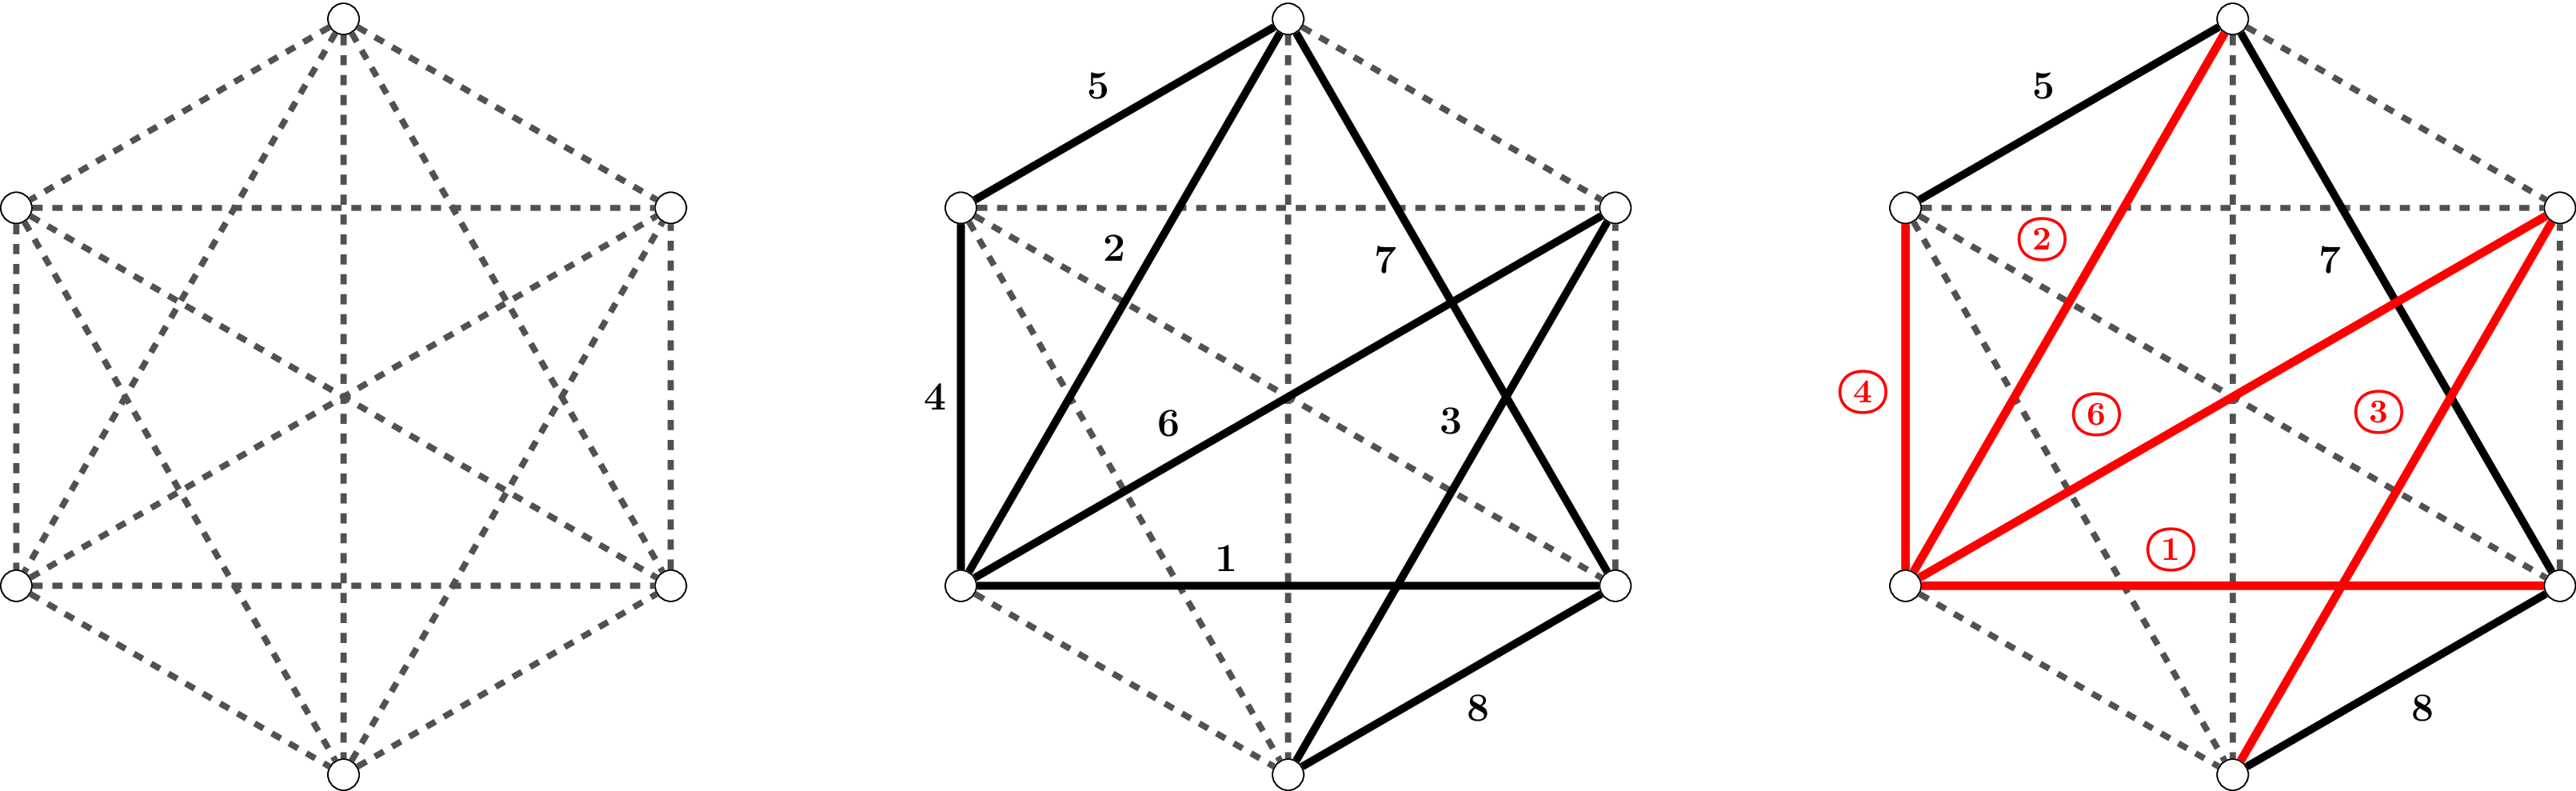
\includegraphics[width=0.9\textwidth]{plow_img.png}
\end{center}
\vspace{10pt}

The king has decided on the number of roads to upgrade, but he is not sure how to label them, so he has turned to Barney (the kingdom's mathematician) to help decide. However, the king is unaware that Barney is actually invested in Mr. Plow, so Barney will choose the set of roads to upgrade and how to label them so that the total cost is as large as possible. What is the maximum cost of plowing the roads?


\section*{Input}

The input consists of a single line containing two integers $n$~($2 \leq n \leq 1\,000\,000$), which is the number of cities, and $m$~($n-1 \leq m \leq \frac{n(n-1)}{2}$), which is the number of roads to be upgraded.


\section*{Output}

Display the maximum possible cost of plowing the roads following the rules above.

